\chapter*{Задание}
Заданием данной лабораторной работы является создание модели для придуманного объекта. В качестве моделируемого объекта была выбрана защита студентами НИР.

На защиту приходит весь поток студентов. Для возможности защиты им необоходимо сначала пройти нормконтроль. Нормконтроль производится за $3-5$ минут и проходится успешно с вероятностью $0,7$. Если результат нормконтроля отрицательный, студет отправляется обратно в очередь, исправлять РПЗ. Если студент проходит нормконтроль успешно, то он готов к защите и ожидает пока освободится одна из комиссий. Если свободны обе комиссии, студент идет к 1-ой. 1-ая комиссия принимает студента за $5-10$ минут и засчитывает ему НИР с вероятностью $0,9$. 2-ая комиссия принимает студента за $30-40$ минут и засчитывает ему НИР с вероятностью $0,1$. Несдавшие студенты отправляются на защиту в другой день.

Процесс моделируется для 120 студентов.

\begin{figure}[h]
	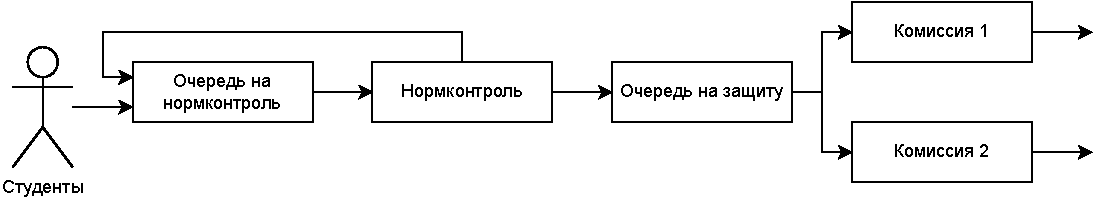
\includegraphics[width=1\linewidth]{"inc/img/Структурная модель.drawio.pdf"}
	\caption{Структурная схема модели}
	\label{s1}
\end{figure}